\documentclass{article}

\ifx\pdfoutput\undefined
% we are running LaTeX, not pdflatex
\usepackage{graphicx}
\else
% we are running pdflatex, so convert .eps files to .pdf
% pdflatex --shell-escape filename
\usepackage[pdftex]{graphicx}
\usepackage{epstopdf}
\fi

\usepackage{hyperref}
\usepackage{verbatim}
%\usepackage{amsmath}
%\usepackage{lscape}
\usepackage{wrapfig}

\begin{document}

\title{Cortana Manual}

\maketitle

%TODO
%binning vs all vs best - may need to go into separate section
%relation between attribute type and target type
%equations for target type seach condition tests
%double correlation
%multi-label
%search strategy
%result window
%search settings vs search parameters (form by conditions and strategy)
%NEW numerical operators, affect single numeric (or all Target Type settings)
%NEW nominal operator !=
%NEW HistogramWindow
%NEW CrossTableWindow
%NEW PlotWindow

%TODO move to actual Start section + ref CPJ
\section{Before you start}
\label{section:before}
Although Cortana is written in Java, and therefore platform independent, it will behave slightly different on different operation systems and/or platforms.
These differences arise from small variations in the Java Virtual Machines, used in different situations.
The main issue is with 32-bit operating systems (OS).
On such systems the maximum amount of memory the Java Virtual Machine (JVM) can use is around 1600 MegaBytes.
However, the actual amount depends on the amount of RAM available.
The cortana.bat and cortana.sh file included in the Cortana.zip set the maximum amount of memory the JVM can use to 1600 MegaBytes, through the -Xmx option.
The value should, at most, be set to half the amount of available RAM, meaning eg. for a 2GB machine to \emph{-Xmx1000m}.
For 64-bit OSes no such limit exists, and it should be save to remove the -Xmx.
Note that the above means that, especially for 32-bit OSes, not all datasets will fit into memory.
This is a problem particularly relevant to the bioinformatics setting (see section~\ref{usage:bioinformatics}), as some of the background sources used for enrichment are relatively large.
%TODO bioinformatics ref





\section{Preliminaries}
\label{section:preliminaries}
Before giving a detailed description of the functionalities of \emph{Cortana}, it is beneficial to first clarify some of the terms used in the rest of this manual.



\subsection{Dataset}
\label{preliminaries:dataset}
First there is the data that will be used as input.
The data can often best be visualised as a table, or matrix, containing \emph{columns} and \emph{rows}.
The first \emph{row} of the data, the \emph{header}, contains all the names of the columns.
The remaining rows form the so-called \emph{instances}, and describe, for each \emph{instance}, the values for each \emph{column}.
Different authors use different names for the same concepts.
To be clear, a \emph{dataset} describes all data under investigation, and is referred to by some authors as \emph{population}.
The members that constitute a \emph{dataset} are referred to as \emph{instances} or \emph{examples}.
Columns will be referred to as \emph{attributes}, and the \emph{column name} is the \emph{attribute name}.

Currently, two types of files can be loaded into \emph{Cortana}, \emph{arff} files and plain (comma separated) text files.
Both file types provide the data in a matrix form.
\emph{arff} (\emph{Attribute-Relation File Format}) files, however, additionally define the data type, or \emph{attribute type}, of each \emph{attribute} in a section preceding the actual data.
\emph{arff} files are very common in data mining. More on them can be found at \url{http://www.cs.waikato.ac.nz/~ml/weka/arff.html}.



\subsection{Attribute Type}
\label{preliminaries:attribute-type}
Each \emph{attribute} has an \emph{attribute type} that indicates what kind of data is associated with the \emph{attribute}.
Currently, \emph{Cortana} distinguishes three \emph{attribute types}: \emph{nominal}, \emph{numeric} and \emph{binary}.
This is less than the number of \emph{attribute types} that can be declared in an \emph{arff} file.
Some of the valid `\emph{arff} types' are mapped to a valid \emph{Cortana} \emph{attribute type}.
For instance, the `\emph{arff} types' \emph{numeric}, \emph{real} and \emph{integer} are all handled by \emph{Cortana} as the \emph{numeric} \emph{attribute type}.
An \emph{attribute} with the \emph{nominal} \emph{attribute type} is said to be a nominal \emph{attribute}, and likewise for the other \emph{attribute types}.
%String and date are not supported atm.



\subsection{Subgroup}
\label{preliminaries:subgroup}
A \emph{subgroup} is a selected number of \emph{instances} from the \emph{dataset}.
As returned by \emph{Cortana}, it will both be non-empty, and will not contain all \emph{instances} in the \emph{dataset}.
Any \emph{Subgroup Discovery} process will try to find \emph{subgroups} that, on a characteristic of interest, show a statistically unusual deviation from the whole \emph{dataset}.



\subsection{Subgroup Discovery}
\label{preliminaties:subgroup-discovery}
\emph{Cortana} is a generic \emph{Subgroup Discovery} tool.
However, it differs from other such tools in some respects.
Traditionally, \emph{Subgroup Discovey} could be described as a heuristic search process in which one tries to optimise for a single \emph{target attribute}, or \emph{target value}, using some \emph{quality measure}.
A \emph{target attribute}, or \emph{target} for short, should be understood as one of the \emph{attributes} available in the \emph{dataset}, and the \emph{target value}, then, is one of the valid values for that \emph{attribute}.

Note that for \emph{nominal} \emph{targets} the \emph{target value} is contained in the data as one of its values.
For a \emph{numeric} \emph{target} however, one does not set a \emph{target value} in \emph{Cortana}, and the underlying \emph{Subgroup Discovery} algorithm will, within the range determined for that \emph{target}, infer its own boundaries to create \emph{subgroups}.
%reference boundary selection process



\subsection{Condition}
\label{preliminaries:condition}
A \emph{condition} is a description, or the intension, of a \emph{subgroup}, while the actual \emph{instances} that form a \emph{subgroup} constitute its extension.
The simplest, or atomic, \emph{condition} consists of three parts: an \emph{attribute}, an \emph{operator} and a value.
More complex \emph{conditions} can be formed from conjunctions of atomic \emph{conditions}.
\emph{Conjunctions} formed this way are sometimes also referred to as \emph{condition lists}.
An example of an atomic \emph{condition} would be: $age \leq 18$, a more complex one would be $age \leq 18 \wedge length \leq 1.8$.



%TODO \Subsection{Operators} on Operators for different AttributeTypes



%TODO nr measures > 43
\subsection{Quality Measure}
\label{preliminatier:quality-measure}
In \emph{Subgroup Discovery}, one uses a \emph{quality measure} to asses the quality of the \emph{subgroups} found.
Here, \emph{quality} should be understood as a score obtained by appying the \emph{qualitiy measure} to, the characteristics of, the \emph{subgroup}.
It depends on the actual \emph{quality measure}, and/or the goal the researcher has in mind, whether such a \emph{quality} should evaluate high or low.
For example, if the very simple \emph{quality measure} `\emph{average}' is used, it depends on the domain specific goal whether one would try to obtain a very high or low score.
\emph{Cortana} features more than 40 \emph{quality measures}, most based on statistical tests.
This manual currently does not provide a description of them, and the user is referred to any statistical handbook, or relevant papers from the data mining community, e.g. \cite{shb,remauv}.
%book



\subsection{Target Attribute vs. Target Concept}
\label{preliminaries:target-concept}
Traditionally, \emph{Subgroup Discovery} focussed only on optimising for a single \emph{target}, or \emph{target value}.
Obviously, this is a setting that can still be used in \emph{Cortana}.
However, since \emph{Cortana} can also be used in a novel setting referred to as \emph{Exceptional Model Mining} (\emph{EMM}) \cite{emm,sdmbn}, the object of optimisation need no longer be singular, and hence non-plural terms like \emph{target} and \emph{target value} are no longer applicable.
Therefore the term \emph{target concept} is introduced.
In better describes what is the object of the optimisation effort used in the \emph{Subgroup Discovery} process.
There are a number of \emph{target types} related to \emph{target concepts}.
Section \emph{Target Type}~\ref{preliminaries:target-type} describes them in more detail, including their influence on the \emph{Subgroup Discovery} algorithm used by \emph{Cortana}.



\subsection{Target Type}
\label{preliminaries:target-type}
%relation between attribute type and target type

\subsubsection{Single Nominal}
The first \emph{target type} is \emph{single nominal}.
It may very well be the best known, and most used, \emph{target type} in the \emph{Subgroup Discovery} discipline.
In this setting, the \emph{target concept} is simply one of the values of the \emph{target attribute}, more commonly known as \emph{target value}.
For most \emph{quality measures}, \emph{Cortana} will optimise the quality of \emph{subgroups} by considering the proportion of positive and negative examples in the \emph{dataset}.
\emph{Instances} count as positive examples if their value for the \emph{target attribute} is identical to the \emph{target concept}, they are negative otherwise.
Note that this yields a binary distinction, such that, for any \emph{target attribute}, only that value that coincides with the \emph{target concept} is considered positive, all other values, including \emph{missing values}, are considered negative.
%TODO So \emph{Cortana} uses the following equality test to determine whether an \emph{instance} is a positive example: \emph{instance.target-attribute.target-value equals target-concept}.
%TODO equals is =, or ==, also adres NEW != operator for NOMINAL

\subsubsection{Single Numeric}
The second \emph{target type} is \emph{single numeric}.
This is another simple \emph{target type}, however, it substantially differs from the \emph{single nominal} type.
Most importantly, one does set a single \emph{target attribute}, but one does not set a \emph{target value} when using this setting.

This \emph{target type} can only be used for \emph{numeric} \emph{attributes}.
All values of such \emph{attributes} are numeric, and thus define a range.
The goal of the \emph{Subgroup Discovery} process will then, most often, be to find a certain threshold value, within that range, that best separates the whole \emph{dataset} into a \emph{subgroup} and its complement, such that the distribution, on the \emph{target attribute}, of that \emph{subgroup} differs most from the distribution of the whole \emph{dataset}.
Here the \emph{quality measure} plays an important role, since it determines whether \emph{Cortana} should try to find \emph{subgroups} that have a much higher or lower average value for the \emph{target attribute} than the average value for the whole \emph{dataset}.
The simple \emph{quality measure} `\emph{average}'  would try to miximise this value, while `\emph{inverse average}' would try to minimise it.

As alluded to above, in this \emph{target type} setting, threshold values are inferred to form \emph{subgroups}.
For a \emph{numeric attribute}, \emph{Cortana} will test various threshold values to set apart \emph{instances}, constituting a new \emph{subgroup}, from the rest of the \emph{dataset}.
Instead of an (in)equality test, as used in the \emph{single nominal} setting, \emph{Cortana} uses can use, a combination of, different tests (`$<=$', `$>=$' and `$=$') to form \emph{subgroups} in the \emph{single numeric} setting.
So, for a \emph{numeric attribute}, a threshold value is selected, and then, for each \emph{instance} in the \emph{dataset}, it is determined whether this \emph{instance} is to be regarded as a positive or a negative example, based on the value of that \emph{instance} and the actual test performed.
Eg., when using the `$<=$' test, an \emph{instance} counts as a positive example if its value is less than, or equal to, the selected threshold, and negative otherwise.
Obviously, in case of the `$>=$' test an \emph{instance} is regarded a positive example if its value is greater than, or equal to, the selected threshold, and considered a negative example otherwise.

The final point to address for this \emph{target type} is to clarifying how \emph{Cortana} actually determines the thresholds it uses.
Unfortunately, there is no short answer to this question, as it depends on the actual \emph{search strategy} selected by the end user.
However, for all three \emph{best numeric} \emph{search strategy} types, \emph{Cortana} selects as threshold a value from the data range of the \emph{numeric attribute} under consideration.
For more details on \emph{search strategy}, see section~\ref{main:search-strategy}.
%binning vs all vs best - may need to go into separate section

\subsubsection{Double Correlation}
This \emph{target type} is used in one of \emph{Cortana's} implementations of possible \emph{Exceptional Model Mining} extentions of traditional \emph{Subgroup Discovery}.
More on \emph{Exceptional Model Mining} in general, and some of its possible implementations, can be found in Leman, Feelders, Knobbe (2008)~\cite{emm}, and the ideas presented there will not be reiterated in this manual.
However, as the purpose of this manual is to provide some useful, or necessary, information about, parts of,  \emph{Cortana}, a little will be said about this \emph{target type}, its use, and the way it influences the \emph{Subgroup Discovery} process used by \emph{Cortana} to form candidate \emph{subgroups}.
%TODO

\subsubsection{Multi-label}
%TODO


\section{Starting Cortana}
After obtaining and unpacking a copy of \emph{Cortana} from \url{http://datamining.liacs.nl/cortana.html}, navigate to the Cortana directory.
There you will find a cortana.jar file.
One could start \emph{Cortana} by double clicking the jar, however, it is recommended to start \emph{Cortana} from the command line.
This way, a lot more information about the \emph{Subgroup Discovery} process is fed back to the user.
To start \emph{Cortana} this way, open a terminal or command window, navigate to the Cortana directory containing cortana.jar, and type: \emph{java -jar cortana.jar}.
Alternatively one can use either cortana.bat (for Windows) or cortana.sh (Bash shell script).
Be sure to read Section~\ref{section:before} \emph{Before you start} if you do.

After starting \emph{Cortana} one is asked to select the file that contains the dataset to be analysed, after which \emph{Cortana}'s main screen is shown.

%TODO implement quickie separator guess code
Currently, two types of files can be loaded into \emph{Cortana}, \emph{arff} files and plain (comma seperated) text files.
The first is very common in data mining and describes the data and additionally defines the \emph{attribute type} of each \emph{attribute}.
As such, \emph{arff} files are preferred over plain text files.
For text files, \emph{Cortana} wil try to infer the correct attribute type of each attribute.
Unfortunately, this may fail, so to check whether Cortana was able to infer the correct attribute type, or change the attribute type anyway, the \emph{Meta Data...} button on the main screen gives access to the \emph{Meta Data Window} (section~\ref{section:meta-data-window}).





\section{Cortana - Main Screen}
\label{section:main}
The main screen of \emph{Cortana} is devided into four major panels, \emph{Dataset}, \emph{Target Concept}, \emph{Search Conditions}, and \emph{Search Strategy}.
The following subsections will address them all.

\begin{figure}
\begin{center}
\centering
\resizebox{1\columnwidth}{!}{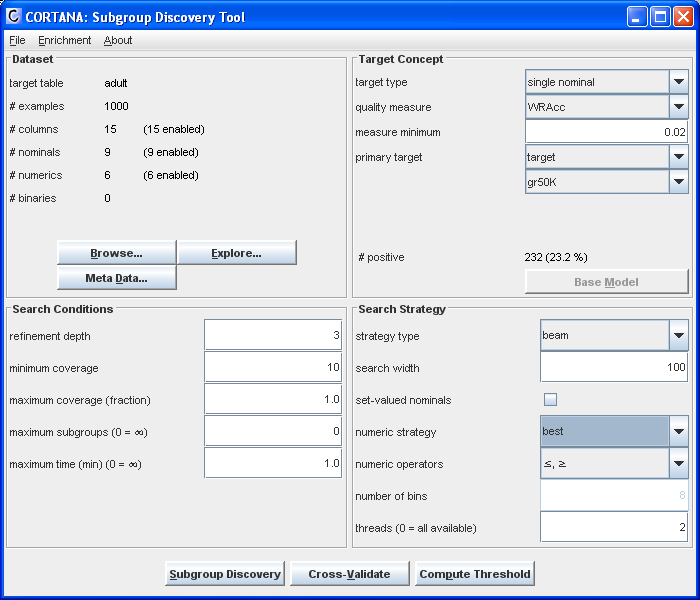
\includegraphics{mainwindow.png}}
\caption{Cortana's main window.}
\end{center}
\label{fig:mainwindow}
\end{figure}


\subsection{Dataset}
\label{main:dataset}
As can be expected from the name, this panel gives some information about the dataset that is currently loaded.

{\bf target table} shows the name of the data file used, which for text files is just the filename, and for ARFF files is the name defined in the '@relation' field.

{\bf\# examples} shows the number of example in the dataset.

{\bf\# columns} shows the number of columns in the dataset.
Remember that columns are also be referred to as attributes.

Finally, there is a number of fields that indicate the number of attributes from each data type.
The type of an attribute determines the sort of mining algorithm or quality measure that is applicable to it.
More about this can be found in section~\ref{preliminaries:attribute-type}.

In addition to the fields described above, there are three buttons present on the Dataset panel, {\bf Browse...}, {\bf Meta Data...} and {\bf Explore...}.

By clicking the {\bf Browse...} button, a {\bf Browse Window} (section~\ref{section:browse-window}) is presented, showing a table with the data in the state that it is currently in.
Additionally, in the table header, it shows the number of distinct values for each attribute.
Note that the data may not be in the same state as when it was loaded, as it can be modified using functionalities of the {\bf Meta Data Window}, presented after pressing the {\bf Meta Data...} button, which is also present on the {\bf Dataset} panel.
Section~\ref{section:meta-data-window} describes the Meta Data Window, its components, and the data manipulation functionalities, in more detail.
To be able to explain them more thoroughly though, it is benefical to describe the various fields of the {\bf Target Concept} panel first.

Explore button.

\begin{figure}
\begin{center}
\centering
\resizebox{0.5\columnwidth}{!}{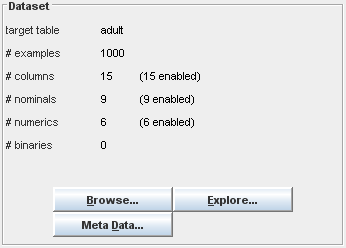
\includegraphics{dataset.png}}
\caption{Dataset details in the main window.}
\end{center}
\label{fig:dataset}
\end{figure}





\subsection{Target Concept}
\label{main:target-concept}
%TODO clean up, contains double info
The fields of this panel serve to manipulate the target concept-related search settings used during the Subgroup Discovery process.
Traditionally, Subgroup Discovery focussed only on optimising for a single target or target value.
Obviously, this is a setting that can still be used in Cortana.
However, since Cortana can also be used in a novel setting referred to as \emph{Exceptional Model Mining} (\emph{EMM}) \cite{emm}, the term target value is no longer applicable, hence the term \emph{Target Concept}.
Section~\ref{preliminaries:target-type} describes the various target types in more detail, including its relation to the type of search strategy (section~\ref{main:search-strategy}) adopted by the Subgroup Discovery algorithm used by Cortana.
In this section only a short description of the various fields will be given.

The first field is {\bf target type}, that, obviously, is used to change the target type for which one wants to do the Subgroup Discovery.
Selecting another target type from the drop down box will force Cortana to consider other attributes as target concept.
For example, when changing the target type from the default single nominal to single numeric, the first attribute having the numeric attribute type is selected, and subsequently displayed in the {\bf primary target} drop down box (see below).

Based on the target type selected, a number of \emph{quality measures} is available.
These are listed in the {\bf quality measure} drop down box.
After changing the \emph{target type}, the \emph{quality measures} listed in the \emph{quility measure} drop down box are automatically updated, to fit the new \emph{target type}.

%TODO explain use of `compute threshold' button
The text field next to \emph{measure minimum} will, by default, show a minimum threshold value for the selected \emph{quality measure}, that, based on historical observations, is considered to be sensible.
One might consider lowering this value if a \emph{Subgroup Discovery} experiment, run with the default value, did not return any, or only few, \emph{subgroups}.
On the other hand, one can increase this value to force \emph{Cortana} to only report \emph{subgroups} that have a quality, as calculated by the selected \emph{quality measure}, that lies above this threshold.
Also, it is worth mentioning that if the search depth is greater than one, leading to conjunctions of \emph{conditions} to be used to select \emph{instances} from the \emph{dataset} to form \emph{subgroups}, the number of intermediate results, when going from one search depth to a higher one, can be lower when using a higher threshold.
This, naturally, aleviates the computational burden of the \emph{Subgroup Discovery} process.
However, the recommended way of controling the amount of (intermediate) results, is through the \emph{maximum subgroups} setting in \emph{Search Conditions}.
More on search depth, or \emph{refinement depth}, and \emph{maximum subgroups} can be found in section~\ref{main:search-conditions} below.

\begin{figure}
\begin{center}
\centering
\resizebox{0.5\columnwidth}{!}{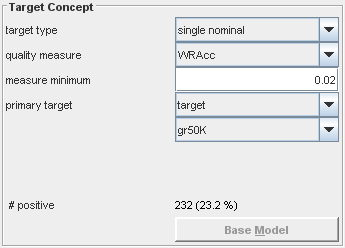
\includegraphics{targetconcept.png}}
\caption{The target concept specification details in the main window.}
\end{center}
\label{fig:targetconcept}
\end{figure}


\begin{comment}
It might be better to present the following fields on a per terget type basis, mentioning, for each target type, only the relavant fields, and their characteristics in relation to that target type.
In code, do not show double correlation if #numerics < 2.
Also, for secondary target select 2nd numeric attribute by default, not first.
In code, do not show multi-label if #binaries < 2.
In code, do not show irrelevant target types based on data set characteristics.
In code, maximum time <= 0, means unlimited time, like in ...
\end{comment}



The items described in the remainder of this section will not be available in every \emph{target type} setting, as the various \emph{target types} are related to the \emph{attribute type} of the \emph{target concept}.
For each item, it will be mentioned to which \emph{attribute type} it applies.

\textbf{primary target} is available in the following \emph{target type} settings: \emph{single nominal}, \emph{single numeric} and \emph{double correlation}.
The \emph{primary target} drop down box lists all \emph{attributes} available in the \emph{dataset}.

\textbf{target value} is available only in the \emph{single nominal} setting.
The \emph{target value} drop down box lists all values of the \emph{attribute} set as \emph{primary target}, which can be of the \emph{nominal} and \emph{binary} \emph{attribute type}.

\textbf{secondary target} is available only in the \emph{double correlation} setting.
In this setting only \emph{attributes} of the \emph{numeric} \emph{attribute type} will be listed in both the \emph{primary target} and \emph{secondary target} drop down box.

%TODO \section{Targets and Settings}
\textbf{targets and settings} is available only in the \emph{multi-label} setting.
If this \emph{target type} is selected, the \emph{Targets and Settings} button will be enabled, and this gives access to the \emph{Multi-label details}.
The upper part of which shows some input fields related to \emph{multi-label} search settings.
The lower part lists all \emph{attributes} of the \emph{binary} \emph{attribute type}.
More on the \emph{multi-label} can be found in section~\ref{section:multi-label} and in \cite{emm,sdmbn}.

Then, there is an information field that shows information relevant to the selected \emph{target type}.
The number of positives, \emph{\# positives} is shown for the \emph{single nominal} \emph{target type}, \emph{average} for \emph{single numeric}, \emph{correlation} for \emph{double correlation} and \emph{\# binary targets} for \emph{multi-label}.

%TODO \Section{Base Model}
The \textbf{Base Model} button will only be enabled if the \emph{target type} is \emph{double correlation} or \emph{multi-label}.
It gives access to a \emph{Base Model Window}, showing a correlation plot for the selected \emph{primary target} and \emph{secondary target}, if the \emph{target type} is \emph{double correlation}.
For the \emph{multi-label} \emph{target type}, it will show a \emph{bayesian network}, connecting the various \emph{binary} \emph{attributes}.







\subsection{Search Conditions}
\label{main:search-conditions}

The fields on this panel allow setting the \emph{search conditions} used in the \emph{Subgroup Discovery} process.
For all fields the default values are also given.

\textbf{refinement depth} controls the number of \emph{conditions} that is used to create \emph{subgroups}.
A \emph{refinement depth} of $1$ would lead to \emph{conditions} like \mbox{[$x <= 9.11$]}, while a \emph{refinement depth} of $2$ would allow for the creation of \emph{conditions} like \mbox{[$x <= 1.2 \wedge y >= 3.4$]}.
It is not recommended to set the \emph{refinement depth} to very high values.
In \emph{Subgroup Discovery}, often a depth greater than $4$ or $5$ does not lead to significant improvements of the \emph{measure score} any more, and just increases both the risk if overfitting, and the computational time needed to calculate the result.
The default value is $1$.

\textbf{minimum coverage} sets the lower bound for the size of the \emph{subgroups} that should be reported by \emph{Cortana}, meaning all reported \emph{subgroups} have at least this size.
The default value is set to $10\%$ of the total \emph{dataset} size, which is shown as \emph{\# examples}, see section~\ref{main:dataset} \emph{Dataset} above.

\textbf{coverage fraction} sets the upper bound for the size of the \emph{subgroups} that should be reported by \emph{Cortana}, meaning all reported \emph{subgroups} have at most this size.
The default value is set to $100\%$ of the total \emph{dataset} size, which is shown as \emph{\# examples}, see section~\ref{main:dataset} \emph{Dataset} above.

\textbf{maximum subgroups} is used to control the maximum number of \emph{subgroups} in the result list generated by \emph{Cortana}.
First, this means that the \emph{Result Window} (section~\ref{section:result-window}) will show at most this number of \emph{subgroups}.
%Search width.

But also, as alluded to in the \emph{Dataset} section (\ref{main:dataset} on \emph{measure minimum}, this number also controls the number of intermediate results retained by \emph{Cortana} to form the pool out of which the generation for the next \emph{refinement depth} is formed.
As such, this \emph{Search Condition} parameter has significant influence on the computational demands, as it directly controls the number of combinatorial candidates to be tested during \emph{Cortana}'s \emph{Subgroup Discovery} process.
Without going into the actual algorithm, a small example probably suffices to make this clear.
For a \emph{dataset} consisting of only \emph{nominal} \emph{attributes}, assume $n =$ \emph{maximum subgroups}, and $m =$ \emph{number of attribute-value pairs}, then the number of candidates $c$ to be tested by \emph{Cortana} for the next \emph{refinement depth} iteration is: $c = n \cdot m$.
The default value is $50$.
%TODO calculation is incorrect, especially with new operator settings.
%Mention search strategies.

\textbf{maximum time (min)} will determine the maximum time, measured in minutes, \emph{Cortana} is allowed to search for new \emph{subgroups}.
After this periode \emph{Cortana} will abort the \emph{Subgroup Discovery} process and report all \emph{subgroups} found up until that point.
This means that especially for the \emph{search strategy} (section~\ref{main:search-strategy}) \emph{strategy type} \emph{depth first} a large of the search space will not be explored at all, if the search proces is aborted.
More precisely, only the first \emph{attributes} will have been addressed at that time.
The default value is $1$.

\begin{figure}
\begin{center}
\centering
\resizebox{0.5\columnwidth}{!}{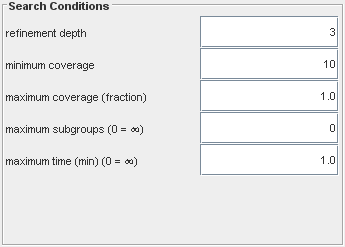
\includegraphics{searchconditions.png}}
\caption{Specification of the searchconditions in the main window.}
\end{center}
\label{fig:searchconditions}
\end{figure}



\subsection{Search Strategy}
\label{main:search-strategy}
%TODO
This is an intro.
It describes \emph{strategy type}, \emph{best numeric} and \emph{number of bins}.

\textbf{strategy type} \emph{beam}, \emph{cover-based beam selection}, \emph{best first}, \emph{depth first} and \emph{breadth first}.
The default value is \emph{beam}.

\textbf{search width} This parameter can not be set for the \emph{best first} \emph{strategy type}.
The default value is \emph{$100$}.

\textbf{numeric operators} The default value is \mbox{\emph{$<=$, $>=$}}.

\textbf{best numeric} \emph{bins}, \emph{best} and \emph{all}.
The default value is \emph{bins}.

\textbf{number of bins} Only available for the \emph{best numeric} setting of \emph{bins}.
Default value is \emph{$8$}.

\begin{figure}
\begin{center}
\centering
\resizebox{0.5\columnwidth}{!}{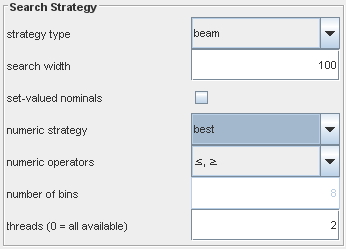
\includegraphics{searchstrategy.png}}
\caption{Search strategy specification in the main window.}
\end{center}
\label{fig:searchstrategy}
\end{figure}






\section{Browse Window}
\label{section:browse-window}
%use of save button in bioinformatics setting (may be made available in every setting to allow saving altered data)
%true positives button in single nominal setting for browse subgroup window
%search

\begin{figure}
\begin{center}
\centering
\resizebox{1\columnwidth}{!}{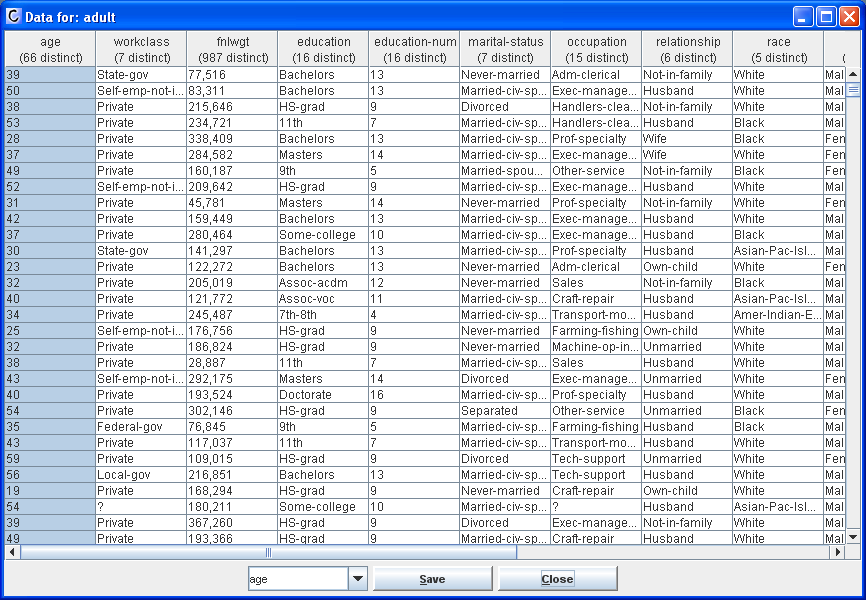
\includegraphics{browsewindow.png}}
\caption{The browse window.}
\end{center}
\label{fig:browsewindow}
\end{figure}




\section{Meta Data Window}
\label{section:meta-data-window}
The \emph{Meta Data...} button gives access to a new window that, next to displaying some additional information about the \emph{dataset} loaded, also allows changing some of the (characteristics of) the data.
The upper part of the \emph{Meta Data Window} shows a table with six columns.
The lower part contains a number of panels that allow modification of the data as it is in memory, note that no modifications are made to the original data file.
First the properties shown in the table in the upper part will be described, the purpose of the various data manipulations will be explained after that.

\begin{figure}
\begin{center}
\centering
\resizebox{1\columnwidth}{!}{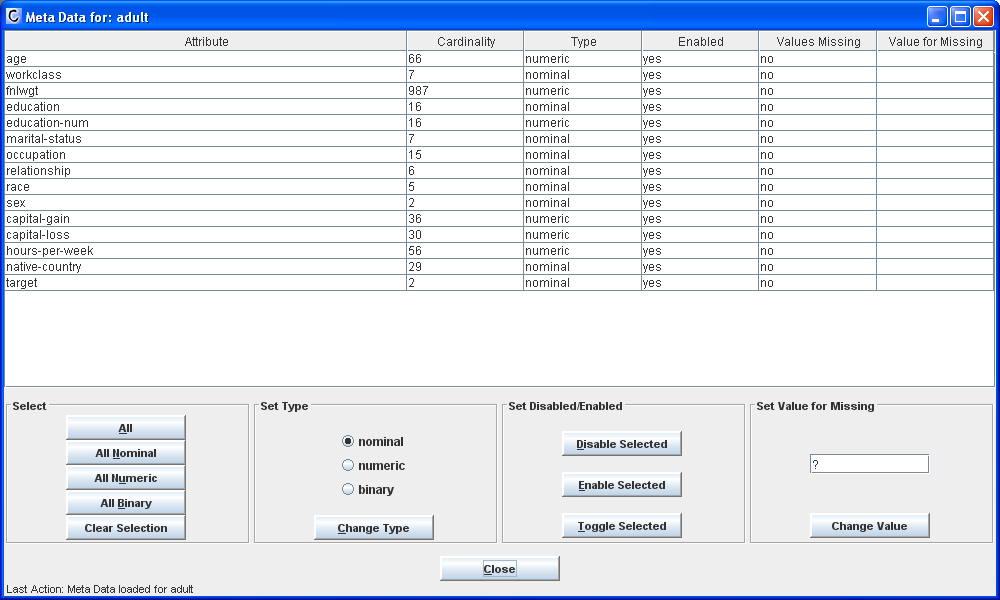
\includegraphics{metadatawindow.png}}
\caption{Meta data window.}
\end{center}
\label{fig:metadatawindow}
\end{figure}



\subsection{Meta Data Table}
\label{meta-data-window:meta-data-table}
The first column in this table, \emph{Attribute}, lists all \emph{attribute names} of the \emph{attributes} in the \emph{dataset}.
The remaining columns show some information for each of these \emph{attributes}.
\emph{Cardiality} gives the number of distinct values for an \emph{attribute}.
\emph{Type} shows its \emph{attribute type}.
\emph{Enabled} indicates whether the \emph{attribute} is \emph{enabled} or \emph{disabled}.
\emph{Values Missing} indicates whether the \emph{attribute} contains missing values or not.
And finally, \emph{Missing Value} shows the value that is currently used for missing values in the data.
Obviously, this field is blank if there are no values missing for the \emph{attribute}.

\subsection{Meta Data Functions}
\label{meta-data-window:meta-data-functions}
The panels in the lower part of the \emph{Meta Data Window} all allow selecting or changing the data.
The first, \emph{Select}, allows selecting all \emph{attributes} of a certain type.
This is a conveiniance method to be used in combination with the functionalities available in other panels.

\textbf{Set Type} allows changing the \emph{attribute type}.
This can be useful for various reasons.
The first is that, after loading a plain text file, it is observed that \emph{Cortana} was not capable to infer the correct type for an \emph{attribute}.
Related to this is the possiblity to change the type of an \emph{attribute} to allow other \emph{quality measures} to be used in the \emph{Subgroup Discovery} process.
An example of this would be an \emph{attribute} that describes the number of doors in a car \emph{dataset}.
If this value is used as a \emph{target value}, one might treat it as a \emph{nominal} property, forcing the \emph{Subgroup Discovery} process to only perform equality tests on this \emph{attribute value} for the creation of the \emph{conditions} used to form \emph{subgroups}.
\emph{Instances} in the \emph{dataset} are then either in the target set if they have the same value for the `doors' \emph{attribute} as the selected \emph{target value}, or are in the complement of the set formed by those \emph{instances}.
If the `doors' \emph{attribute} is treated as \emph{numeric}, any, combination, of the `$<=$', `$>=$' and `$=$' tests can used to create \emph{conditions} to perform on the \emph{attribute values}.
This means that the size of the set of \emph{instances} selected using an \emph{attribute value} might be bigger than in the \emph{nominal} case.
A \emph{condition} using \mbox{[$doors >= 2$]} will select all cars having two or more doors.
In the \emph{nominal} case it would not be possible to select this group using only one \emph{condition} (assuming the set of cars having more than two doors is not empty).
Obviously, it would be possible to select the same group using a set of \emph{conditions} like \mbox{[\emph{doors equals `$2$' $\vee$ doors equals `$3$' \ldots}]}, but, among other negative characteristics, creating such \emph{conditions} would be computationally more demanding, and less intuitive.
Note that if there are missing values for an \emph{attribute}, the \emph{missing value} value for this \emph{attribute} might be automaticaly changed to a value that is relevant to the \emph{attribute type}.
See \emph{Set Value for Missing} below for more on the \emph{missing value} values for the different \emph{attribute types}.
%\ref{subsubsection:set-missing-values}

\textbf{Set Disabled/Enabled} allows to disable or enable an \emph{attribute}.
When an \emph{attribute} is disabled, it will not be considered by the mining algorithm to form \emph{conditions} with to create \emph{subgroups}.
Note that disabling an \emph{attribute} does not affect the possiblity to select it as a \emph{target concept} (see section~\ref{preliminaries:target-concept} for more on \emph{target concepts}).

\textbf{Set Value for Missing} can be used to change the value that is curently used for values that were missing in the data.
The value that is used for missing values depends on the type of the \emph{attribute}.
If, in an \emph{arff} file, values are declared missing, using the `\emph{?}' directive, \emph{Cortana}'s file loader might replace this value with one that makes more sense in its \emph{Subgroup Discovery} setting.
For \emph{nominal} types it will leave this value as is.
This will result in `\emph{?}' being one of the possible \emph{target values} one can select for the corresponding \emph{attribute}.
However, one can assign a diffent value to the \emph{missing values}.
One than has two options, either assign the \emph{missing values} a value that is an existing one for the \emph{attribute}, or a non-exiting one.
In the first case one effectively assigns all \emph{instances} that have a missing value for the corresponding \emph{attribute} to one of the other \emph{attribute values}.
In the latter case, one just changes the value.
When changing the \emph{missing value} value of an \emph{attribute}, the \emph{Cardinality} column is updated accordingly.
For \emph{numeric} and \emph{binary} \emph{attribute types} \emph{Cortana}'s file loader will replace `\emph{?}' values with $0.0$ and $false$, respectively.
Again, if this is incorrect, or one wishes to assign the \emph{missing values} another \emph{attribute value}, either existing or non-existing, this can be done analogously to the \emph{nominal} case.
%Mention automatic missing value update on attribute type change.
%TODO valid values for each AttributeTypes





%TODO
\section{Multi-label}
\label{section:multi-label}





\section{Result Window}
\label{section:result-window}
When a mining run terminates, a \emph{Result Window} is shown.
The titlebar of this window shows some basic information about the search settings that were used to obtain the result displayed.
The top half of a \emph{Result Window} shows a table with the \emph{subgroups} found, the lower half contains two rows of buttons.
Some of the buttons on this \emph{Button Panel} will be presented only in certain search settings.
Also, a number of buttons is used for post-processing, others just give access to additional information.
Finally, the buttons in the lower row will execute operations on the whole \emph{Result Set}, that is all results shown in the \emph{Result Window}, while those in the upper row operate only on the selected \emph{subgroup(s)}.

The following subsections will go into detail about the use of the various components of the \emph{Result Window}.

\begin{figure}
\begin{center}
\centering
\resizebox{1\columnwidth}{!}{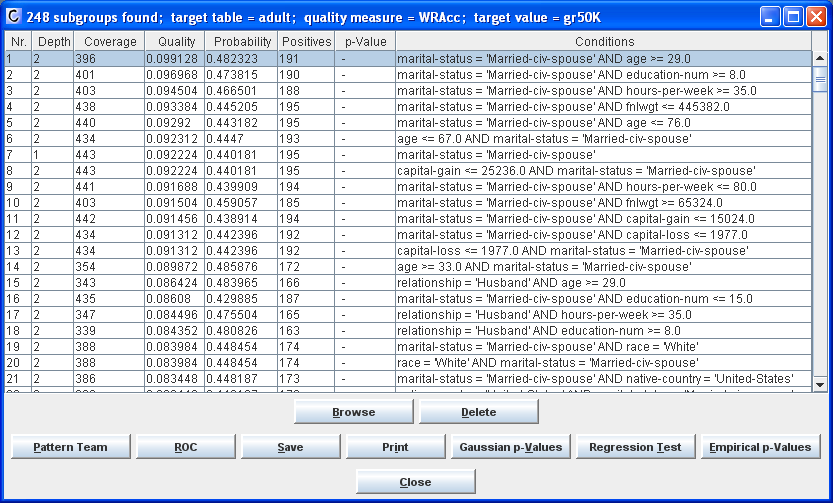
\includegraphics{resultwindow.png}}
\caption{The result window.}
\end{center}
\label{fig:resultwindow}
\end{figure}


\subsection{Result Set Table}
\label{result-window:result-set-table}
The top half of the \emph{Result Window} consists of a \emph{Result Set Table}, showing all \emph{subgroups} in the \emph{result set}.
Form left to right the columns in this table are: \emph{Nr.}, \emph{Depth}, \emph{Coverage}, \emph{Measure}, \emph{p-Value} and \emph{Conditions}, and they all reveil a characteristic of the \emph{subgroup} found.
This section will address all columns, and explains how to interpret the information they display.

\emph{Nr.} shows the rank of the \emph{subgroup}.
Note, however, that \emph{Cortana} does not use a partial ranking for ties, and, as a result, \emph{subgroups} that attain the same \emph{measure} score, will not receive equal ranks.
Rather, if such an event occurs, \emph{Cortana} assigns the value, displayed by \emph{Nr.}, based on where in the \emph{Subgroup Discovery} process the \emph{subgroup} was found.

\emph{Depth} shows the \emph{refinement depth} at which the \emph{subgroup} was found.
As explained in the section on \emph{Search Conditions} (\ref{main:search-conditions}), the \emph{refinement depth} controls the number of \emph{conditions} that is used to create a \emph{subgroup}.
So, a \emph{subgroup} that is formed by using only one \emph{condition} is said to have been found at depth $1$.
The number displayed at \emph{Depth} is the same as the number of conjuncts in the \emph{Conditions} column of the \emph{Result Set Table}.

Note that in \emph{Subgroup Discovery} it often happens that one \emph{condition} already selects a highly valuable, high scoring, \emph{subgroup}.
Adding extra \emph{conditions} to this first one may improve the \emph{measure} score, but only by a, possibly very, limited amount.
This will lead to a \emph{result set} containing a number of \emph{subgroups} that all consist of the same 'base' \emph{condition}, which is then refined with additional \emph{conditions} using another \emph{attribute}.
If these extra \emph{conditions} do not substantially increase the \emph{measure} score, all of these variations will attain consecutive ranks in the final \emph{result set}.

\emph{Coverage} shows the number of \emph{instances} in the \emph{subgroup}.
Depending on the \emph{target type} used, this number can consist of both \emph{true positives} and \emph{false positives}, or just indicates the total size of the \emph{subgroup}.

\emph{Measure} shows the score of the \emph{subgroup}, according to the \emph{quality measure} used.
Different \emph{quality measures} have different ranges for the scores they asssign to the worst and best possible \emph{subgroups}.
As a result, \emph{measure} scores resulting from applying different \emph{quality measures} can not be compared directly in any sensible manner.
%ref wouter comparison paper

\emph{p-Value} is initially blank.
But it will show the p-value of the \emph{subgroup} after additional user input.
In \emph{Subgroup Discovery}, \emph{quality measures} are used that are based on, or insired by, well known, standard, statistical tests.
However, \emph{Cortana} does not allow calculation of p-values in a fashion that is customary in statistics.
To be able to do so, the \emph{dataset} under investigation should be considered a sample of the total population itself.
But, as the \emph{dataset} is not treated as such, the calculation of the p-value is done using a different paradigm.
The major benefit of this paradigm is that it is agnostic to the \emph{target type} used in the \emph{Subgroup Discovery} process.
Section~\ref{result-window:p} \emph{Compute p-Value} below describes how the p-value is calculated in \emph{Cortana}.
% ref thesis barbara p-value
% ref wouter p-value

\emph{Conditions} shows the \emph{condition(s)} used to form a \emph{subgroup}.
As explained in section~\ref{preliminaries:condition} \emph{Condition}, a \emph{condition} consists of an \emph{attribute}, an operator, and a value.
For depths greater than $1$ \emph{Conditions} shows a conjunction of such \emph{conditions}.



\subsection{Subgroup Buttons}
\label{result-window:subgroup-buttons}
The following subsections describe the various buttons that can appear on the upper row of the lower part of the \emph{Result Window}.
These buttons operate only on the \emph{subgroup(s)} that are selected, or highlighted, in the \emph{Result Set Table}.
The selection can be changed using the mouse or pressing (Shift) and the Down/Up arrow of the keyboard.
The \emph{target type} setting used for the \emph{Subgroup Discovery} experiment determines which buttons will be shown.
For all buttons it will be indicated for what \emph{target type} setting it is applicable.



\subsubsection{Show Model}
\label{result-window:model}
\emph{Show Model} is available only for the \emph{multi-label} \emph{target type}.
For all \emph{subgroups} selected in the \emph{Result Set Table}, it will show a new \emph{Model Window}, depicting the bayesian network connecting the \emph{binary} \emph{attributes}, according to the model that was inferred through the \emph{Subgroup Discovery} process.



\subsubsection{Browse Subgroup}
\label{result-window:browse}
\emph{Browse Subgroup} is available for all \emph{target types} and will show a \emph{Browse Window} as described in the \emph{Browse Window} section (\ref{section:browse-window}).
For all \emph{subgroups} selected in the \emph{Result Set Table}, it will show such a window, depicting all \emph{instances} that constitude the \emph{subgroup}.
For the \emph{single nominal} \emph{target type} one additional button is available, the \emph{True Positives} button.
Clicking it will highlight only those \emph{instances} that count as \emph{true positives}.
%TODO in code: save subgroup possiblility, not only save whole table



\subsubsection{Delete Subgroup}
\label{result-window:delete}
\emph{Delete Subgroup} is available for all \emph{target types} and deletes a \emph{subgroup} from the \emph{Result Set}.
Note that this means that the \emph{subgroup} is removed both from the visible \emph{Result Set Table}, as from the underlying \emph{result set}.
This means that, after deletion, the \emph{subgroup} will no longer show up in the results of the \emph{Save} and \emph{Print} actions described below.
Also, in the \emph{single nominal} setting, this point is no longer used for any ROC plot created after deletion.
ROC plots created before deletion are unaffected.
This is intended behaviour, as in this way it allows comparison of ROC plots of the same \emph{result set} in a way that would not be possible if pre-existing ROC plots are update after any deletion.



\subsection{Result Set Buttons}
\label{result-window:result-set-buttons}
The following subsections describe the various buttons that can appear on the lower row of the lower part of the \emph{Result Window}.
These buttons operate on the whole \emph{result set}, that is, on all \emph{subgroups} in the \emph{result set}.
As such, the results of these operations are unaffected by, changes in, the selection of \emph{subgroups} in the \emph{Result Set Table}.
The \emph{target type} setting used for the \emph{Subgroup Discovery} experiment determines which buttons will be shown.
For all buttons it will be indicated for what \emph{target type} setting it is applicable.


\subsubsection{ROC}
\label{result-window:roc}
\emph{ROC} is only available for the \emph{single nominal} \emph{target type}.
All \emph{subgroups} in the \emph{Result Set Table} will be taken into account to show a \emph{ROC Curve Window}.
ROC (Receiver Operating Characteristic) curves have their origin in electrival engeneering, where they are used to show the performance of classifiers.
In the \emph{single nominal} setting some of the members of a \emph{subgroup} are \emph{true positives}, while others are \emph{false positives}.
In a ROC plot the \emph{true positive rate} (TPR) of each \emph{subgroup} is plotted against its \emph{false positive rate} (FPR).
When this is done, a line, the ROC curve, can be draw that forms a convex hull connecting the outer most points.
A straight diagonal from the lower left corner to the upper right indicates complete randomness of the result, and the furher the line approaches the upper left corner the better the result.
For a \emph{subgroup} to reach the upper left corner, its TPR must be $1$, and its FPR $0$.

\begin{figure}
\begin{center}
\centering
\resizebox{1\columnwidth}{!}{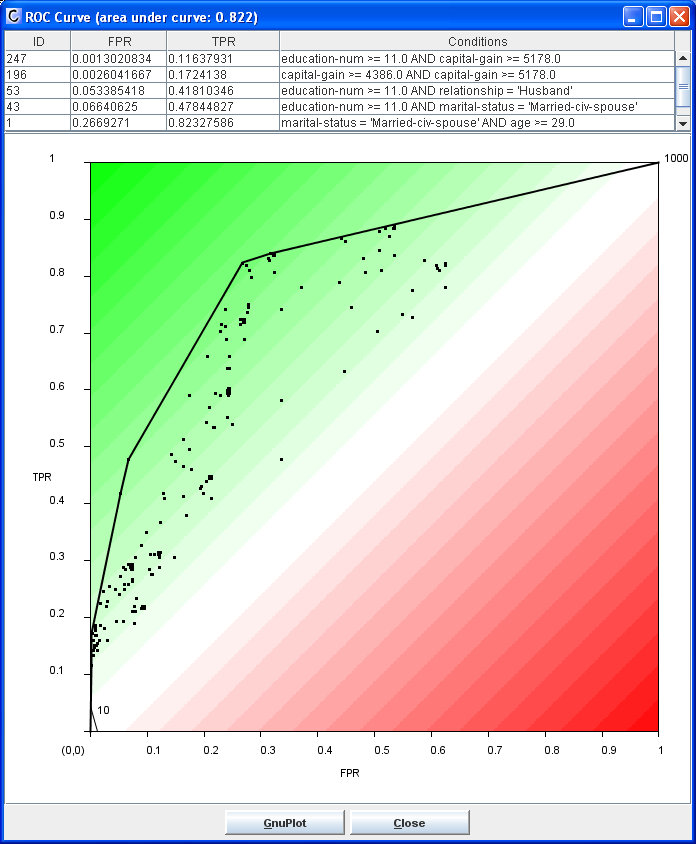
\includegraphics{rocwindow.png}}
\caption{The ROC window.}
\end{center}
\label{fig:rocwindow}
\end{figure}



\subsubsection{Compute p-Values}
\label{result-window:p}
To calculate the p-values for the \emph{subgroups} found, the end user clicks the \emph{Compute p-Value} button on the \emph{Button Panel}.
In short the calculation of p-values is done by creating n random subgroups ...
%TODO explain

\begin{figure}
\begin{center}
\centering
\resizebox{0.3\columnwidth}{!}{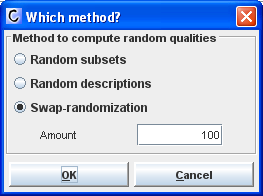
\includegraphics{randomizationdialog.png}}
\caption{Choosing the type of randomization to be used for any significance testing.}
\end{center}
\label{fig:randomizationdialog}
\end{figure}



\subsubsection{Regression Test}
\label{result-window:regression}
TBI.



\subsubsection{Empirical p-Values}
\label{result-window:empirical-p}
This functionality may be removed.



\subsubsection{Fold}
\label{result-window:fold}
TBI.



\subsection{Save}
\label{result-window:save}
\emph{Save} is available for all \emph{target types}.
It allows saving of the whole \emph{result set} to a file.
The user will be asked for a name and location of this file.
The file will contain the information as it is depicted in the \emph{Result Set Table}, and the values for the various columns will be comma separated.
Currently, there is no method of changing this separator.
%TODO in code: if (subgroups selected) 'save' button becomes 'save selected'
%TODO in code: allow CSV,TSV,SemiColonSV through file selector/file type



\subsubsection{Print}
\label{result-window:print}
\emph{Print} is available for all \emph{target types}.
It allows printing of the whole \emph{Result Set Table}.
Note that it does not have a maximum amount of result it prints, the \emph{Result Set Table} will be printed as-is.
Therefore, it is not recommended to use this functionality on large \emph{Result Sets}/\emph{Result Set Tables}.
%TODO in code: if (subgroups selected) 'print' button becomes 'print selected'
%TODO in code: ask for 'print n subgroups'



\subsubsection{Close}
\label{result-window:close}
\emph{Close} is available for all \emph{target types}, and it will close the \emph{Result Window}.
Note that it can not be reopened.
Therefore, all necessary actions like, saving or printing the results, should be done before closing the \emph{Result Window}.
All results will be lost, and the only way to get a new \emph{Result Window} is to run the same \emph{Subgroup Discovery} process again.
As this may be a very lengthy process, be sure to finish all operations before closing the \emph{Result Window}.





\section{Usage}
\label{section:usage}



\subsection{Orinary Subgroup Discovery}
\label{usage:normal}
java -jar Cortana.jar



\subsection{Bioinformatics Setting}
\label{usage:bioinformatics}





\section{Autorun}
\label{section:auto-run}
\emph{Cortana} comes with the ability to run experiments in an unsupervised setting.
This is a mode that is specifically created to allow so-called batch mining.
This section will explain how \emph{Cortana} accomplishes this, and how to set up an \emph{autorun} or batch mining experiment.

In normal usage mode, the end user can set all search settings using the graphical user interface (GUI).
After loading a data file and setting the search settings one usually clicks the \emph{Subgroup Discovery} button, and the \emph{Subgroup Discovery} process begins.
However, \emph{Cortana}'s menu bar on the top of the main window gives access to two options that allow saving the search parameters to a XML-file.
This file can then be used to start the \emph{Subgroup Discovery} process, using the defined search settings, at some other time.

The two autorun related options can be found under \emph{File}, and are named \emph{Create Autorun File} and \emph{Add to Autorun File}.
The first will ask the user for a name and location for the new file that will be created, containing all information, as shown in the main window, needed to do an unsupervised \emph{Subgroup Discovery} experiment.
The second option allows to add all information currently presented by the main window to an already existing \emph{autorun} file.
By using this last option one can create a large file, containing multiple experiments.
An example usage would be running several experiments on a single data file, where each experiment uses a different \emph{quality measure}.

The paragraph above refers to information, and not solely search settings, as the XML-file used in the \emph{autorun} setting also needs to know the name of the data file to use.
That name is not part of the search settings, but it is important to state how \emph{Cortana} looks for this data file.
When loading the \emph{autorun} XML-file, \emph{Cortana} will remember the directory in which this \emph{autorun} file resides.
It will then parse the XML-file, and retrieve the name of the data file to use.
\emph{Cortana} will then try to load the data file from the directory in which the \emph{autorun} resides, and that directory only.
This means no relative paths can be used for the location of the data file, and the \emph{autorun} file should always reside in the same directory as the data file(s) for which it describes experiments.
Although this limits its use, it keeps it easily portable, as, in this way, one can simply exchange directories containing \emph{autorun} file(s) and accompanying data file(s), without having to worry about setting paths correctly in the \emph{autorun} file, or placing the directories in the correct relative location, before being able to run an experiment.

When \emph{Cortana} runs an experiment defined in an \emph{autorun} file, the \emph{Subgroup Discovery} process is exactly the same as when the experiment would be started from the GUI.
However, at the end of the \emph{Subgroup Discovery} process, there are a few deviations from the normal GUI situation.

First of all, when the \emph{Subgroup Discovery} process terminates, the \emph{Result Set} will be automatically saved, as it would happen when the end used clicks the \emph{Save} button in the \emph{Result Window}.
The result file will have a name indicative of the search settings used, and starts with the data file name.
Also, it will contain a time stamp as part of its name, so that identical runs on, updated versions of, the data file will not overwrite older results.
The result file will be saved to the directory in which the \emph{autorun} file resides.
%TODO in code make cleaner autosave file name

Second, a \emph{Result Window} may or may not be shown.
Whether it is, is controlled by a command line parameter, as shown at the end of this section.
Omitting this command line parameter will cause \emph{Cortana} to default to always showing a \emph{Result Window} after an experiment finishes.
Showing the \emph{Result Window} is necessary if one wishes to perform additional actions on the \emph{result set}, be it plotting \emph{ROC Curve Windows}, calculating p-Values or any of the other actions described in section~\ref{section:result-window} \emph{Result Window}.

Third, if the \emph{autorun} file defined multiple experiments, the next experiment will be run automatically.
This will go on until all the experiments in the \emph{autorun} file are executed.
In case of any errors, for example when \emph{Cortana} can not locate a data file, some efforts are made to resume execution by discarding the erroneous experiment and continuing with the next.

A final, more technical, word about the \emph{autorun} files.
The preferred way to create \emph{autorun} files is through the \emph{Cortana}'s main GUI.
In most cases this is the most convenient way, eliminating the chance of errors that could occur when one were to craft an \emph{autorun} file by hand.
The XML-parser parsing the \emph{autorun} file uses a very strict \emph{autorun} definition file, and will throw errors when any of the XML tags are not present in the \emph{autorun} file.
This means that, even for XML-tags that define settings that are not relevant to the experiment for which they are defined, they should be present, although they will be so-called empty tags in such a case.

Note that some efforts were taken to allow \emph{Cortana} to run in a headless environment, as is customary for the majority of servers.
If all goes well, this should not be a problem.
However, if an error occurs, it may cause an error message windows or dialogs to be shown.
Obviously, showing this in a headless environment will fail, and may lead to additional errors.
This is a known problem, but will not be addressed any time soon.

To use \emph{Cortana} in \emph{autorun} mode start it as shown below, where \emph{file.xml} is the \emph{autorun} file to use, and the optional \emph{false} controls whether a \emph{Result Window} should be shown after each experiment finishes.
Remember that the default is \emph{true}, and the second parameter can thus be omitted if one wishes to see the \emph{Result Window}.

java -jar Cortana.jar file.xml [false]





\begin{thebibliography}{10}

\bibitem{shb}
Author,
\newblock{Statistical Handbook}
.

\bibitem{remauv}
Lavrac, Flach, Zupan,
\newblock{Rule Evaluation Measures, a unifying View},
.

\bibitem{emm}
Leman, Feelders, Knobbe,
\newblock \emph{Exeptional Model Mining},
.

\bibitem{sdmbn}
Wouterd,
\newblock{Subgroup Discovery meets Bayesian Networks, an EMM approach}
.

\end{thebibliography}

\end{document}

